
\begin{document}
\abstract{Balanced Scorecard y Business model canvas son técnicas de análisis empresarial . Ambas técnicas son útiles para mejorar el desempeño organizacional. Pero sus aplicaciones difieren. Ambos se pueden usar junto con los indicadores clave de rendimiento para monitorear y mejorar el rendimiento de la organización. Vamos a entender tanto la técnica en detalle.}

 Abstract\\
Balanced Scorecard and Business model canvas are business analysis techniques. Both techniques are useful to improve organizational performance. But their applications differ. Both can be used together with the key performance indicators to monitor and improve the performance of the organization. We will understand both the technique and the detail.
\newpage

\section{Introduccion}
Esta metodología deriva de la gestión estratégica de empresas y presupone una elección de indicadores que no debe ser restringida al área económico – financiera. Así como no es posible comandar un avión controlando apenas la velocidad, los indicadores financieros no son suficientes para garantizar que una empresa se dirija en la dirección correcta. Por estos motivos, será necesario monitorear, junto a los indicadores económicos –financieros, el desempeño de mercado, los procesos internos, la innovación y la tecnología. De este modo, los resultados financieros serán fruto de la sumatoria de acciones generadas por personas a través del uso de las mejores tecnologías, vinculación a las mejores prácticas y los procesos internos de la organización, todo esto en armoníacon la Propuesta de Valor ofrecida al cliente. Esto proceso se denomina "crear valor através de activos intangibles"

\begin{center}
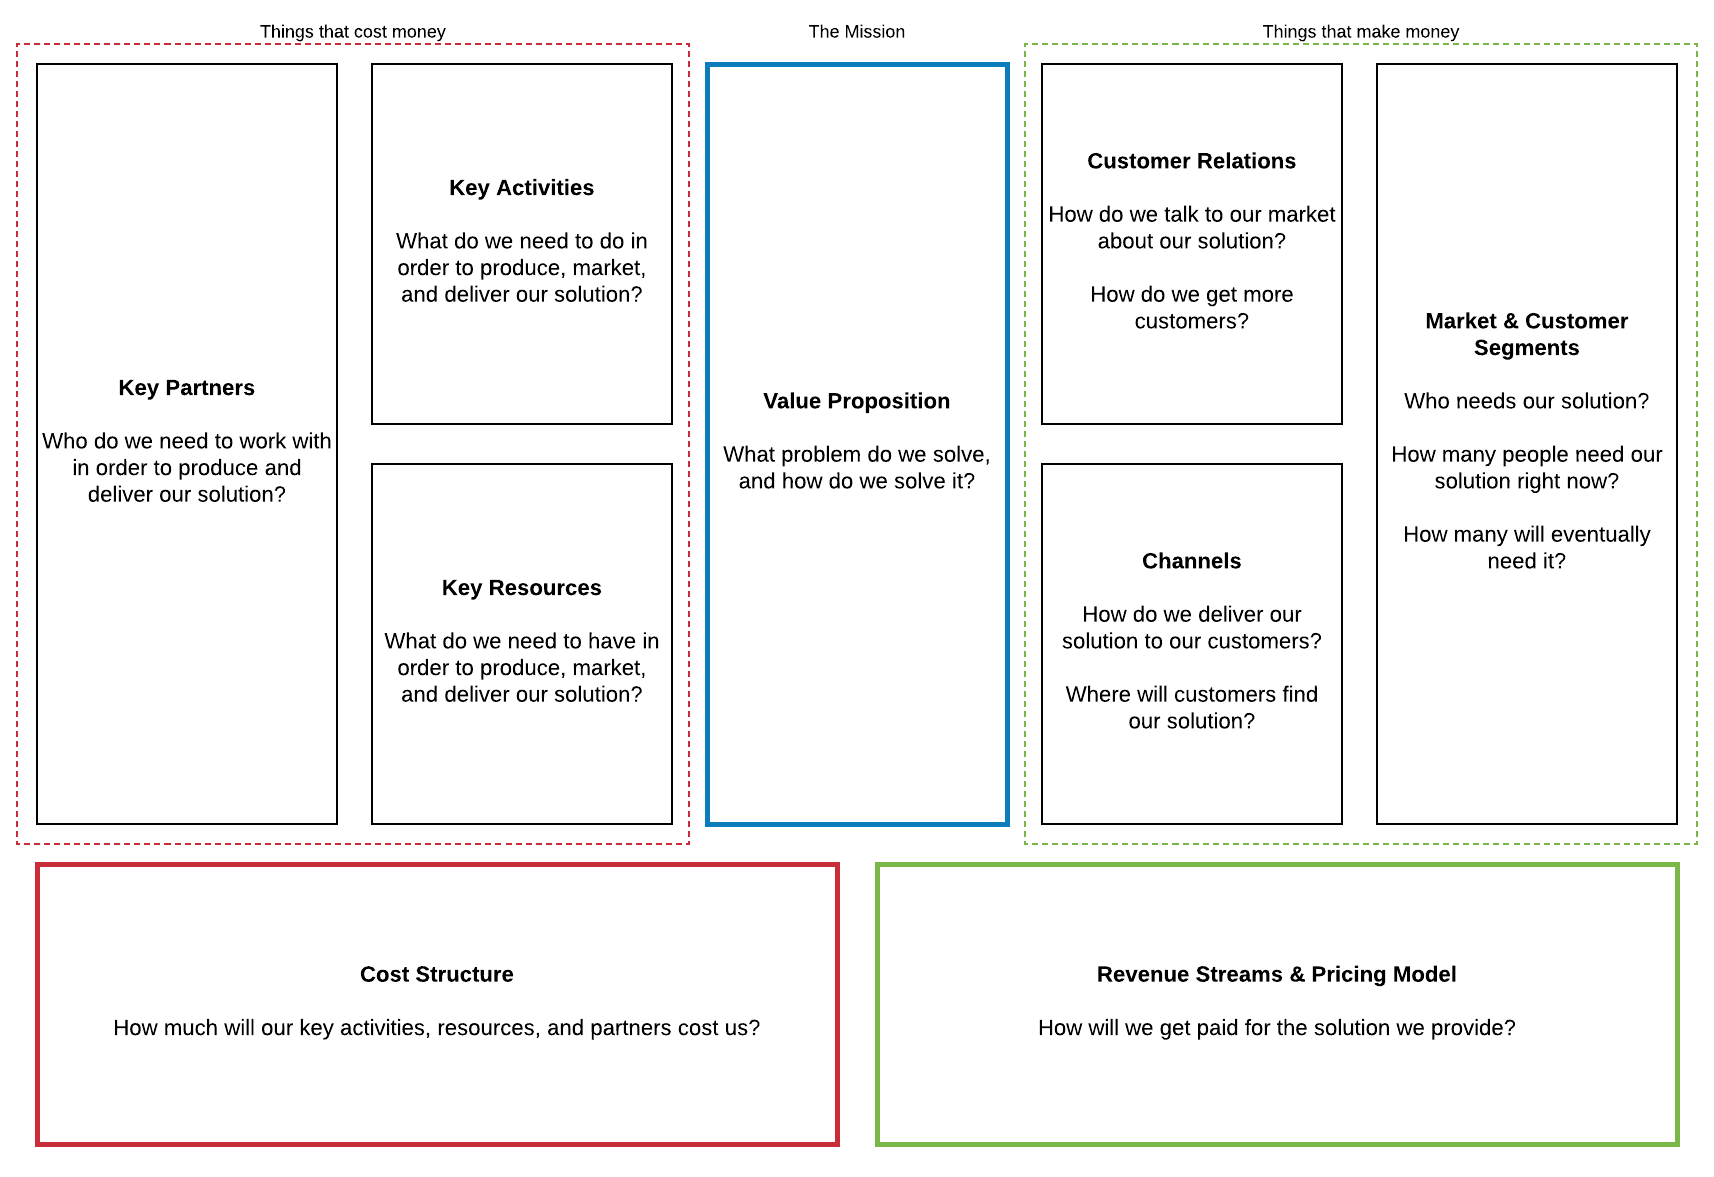
\includegraphics[width=10cm]{./Imagenes/imagen5}
\end{center}

Balanced Scorecard ofrece una visión integrada y balanceada de la empresa y permite desarrollar la estrategia en forma clara. Esto se logra a través de objetivos estratégicos identificados en 4 perspectivas: financiera, clientes, procesos internos yaprendizaje e innovación. Cada una de las perspectivas se vincula con las demás mediante relaciones de causa y efecto. BSC promueve, además, el alineamiento de losobjetivos estratégicos con indicadores de desempeño, metas y planes de acción para hacer posible la generación de estrategias en forma integrada y garantizar que los esfuerzos de la organización se encuentren en línea con las mismas.
\newpage


\section{Balanced Scorecard}
\item{El Balanced Scorecard (BSC) o Cuadro de Mando Integral (CMI) es una herramienta de gestión que permite implementar la estrategia de una empresa a partir de una serie de medidas de actuación, permitiendo un control permanente sobre todos los factores de la organización, interrelacionando objetivos y relacionándolos con acciones concretas.}

\begin{center}
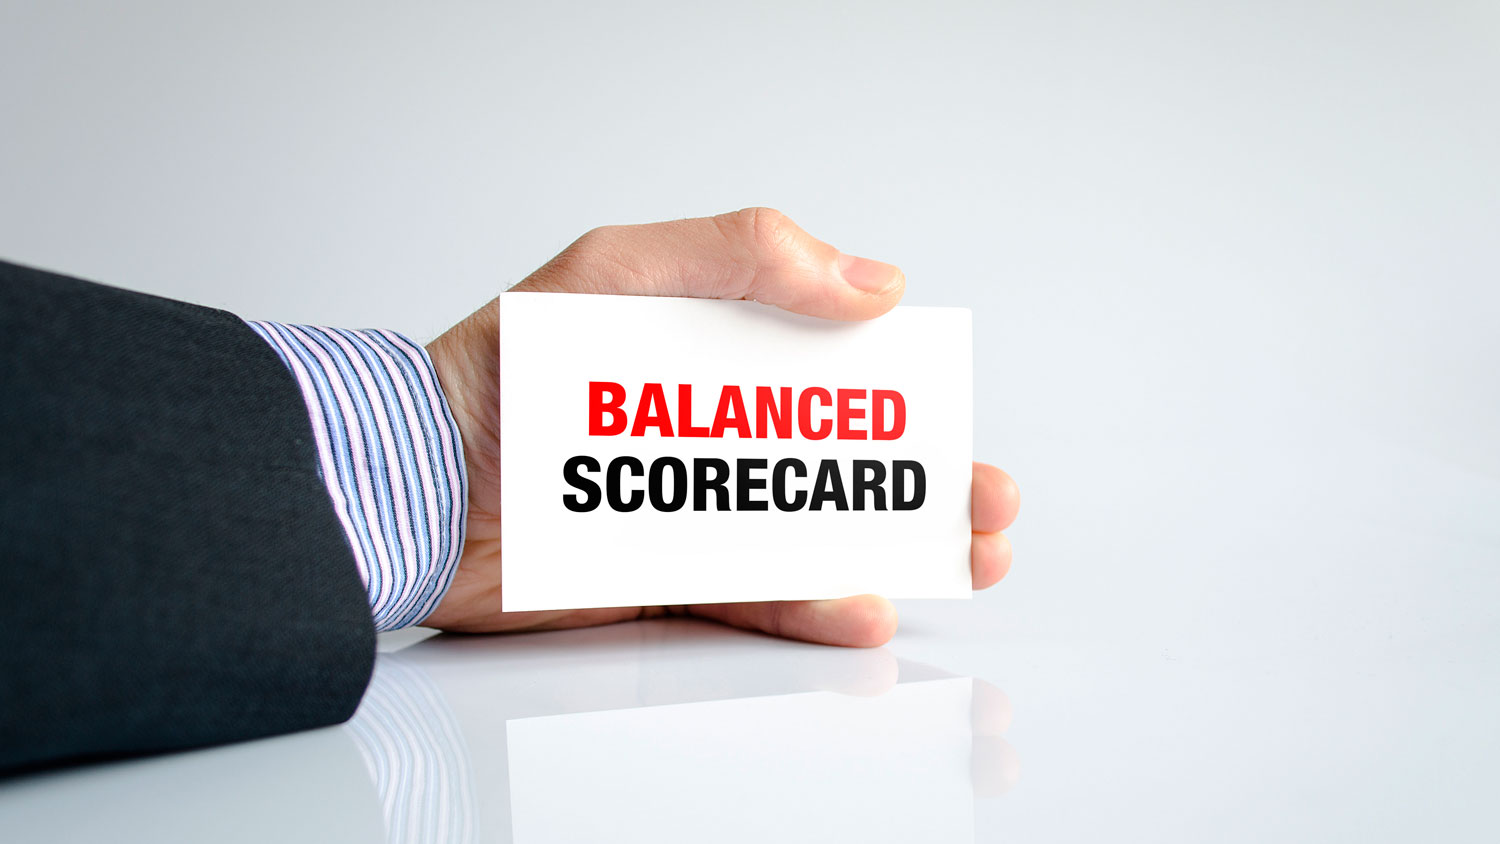
\includegraphics[width=15cm]{./Imagenes/imagen1}
\end{center}

\section{¿Cómo funciona el Balanced Scorecard?}
\item{El proceso de creación de un BSC comienza con la determinación de los siguientes parámetros:\\\\
-Objetivos a alcanzar por la organización.\\
-Indicadores o mediciones más adecuados para poder controlar el grado de alance de los objetivos.\\
-Metas concretas en relación a los resultados específicos de dichas mediciones.\\
-Acciones, iniciativas proyectos o programas que se van a implementar para lograr dichas acciones.\\\\
Una vez fijados todos estos factores, el siguiente paso es colocar todas estas mediciones, metas y objetivos en un panel o cuadro, utilizando para ellos un software específico donde se monitorea el progreso de cada uno de ellos.\\
Los datos, que normalmente se obtienen de los sistemas informáticos de la empresa, se presentan de manera esquemática y muy gráfica en un panel similar al que utilizan los pilotos de aviones, por lo que también se le conoce como «Cuadro de Mando Integral».}

\section{Perspectivas del Balanced Scorecard}
\item{A pesar de que son 4 las perspectivas que tradicionalmente identifican un BSC, no es indispensable que estén todas ellas; estas perspectivas son las más comunes y pueden adaptarse a la gran mayoría de las empresas, y no constituyen una condición indispensable para construir un modelo de negocios.\\\\\

\begin{center}
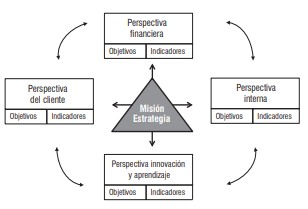
\includegraphics[width=15cm]{./Imagenes/Imagen02}
\end{center}

\textbf{Perspectiva financiera}\\
Históricamente los indicadores financieros han sido los más utilizados, pues son el reflejo de lo que está ocurriendo con las inversiones y el valor añadido económico, de hecho, todas las medidas que forman parte de la relación causa-efecto, culminan en la mejor actuación financiera.Información administrada por un sistema ERP.\\\\
\textbf{Perspectiva del cliente}
Como parte de un modelo de negocios, se identifica el mercado y el cliente hacia el cual se dirige el servicio o producto. La perspectiva del cliente es un reflejo del mercado en el cual se está compitiendo. Brinda información importante para generar, adquirir, retener y satisfacer a los clientes, obtener cuota de mercado, rentabilidad, etc. "La perspectiva del cliente permite a los directivos de unidades de negocio articular la estrategia de cliente basada en el mercado, que proporcionará unos rendimientos financieros futuros de categoría superior." (Kaplan & Norton).
Información administrada por un sistema CRM o BPC.\\\\
\textbf{Perspectiva procesos internos}\\
Para alcanzar los objetivos de clientes y financieros es necesario realizar con excelencia ciertos procesos que dan vida a la empresa. Esos procesos en los que se debe ser excelente son los que identifican los directivos y ponen especial atención para que se lleven a cabo de una forma perfecta, y así influyan a conseguir los objetivos de accionistas y clientes.
Información administrada por un sistema BPC o BPM.\\\\
\textbf{Perspectiva de formación y crecimiento}\\
Es la perspectiva donde más tiene que ponerse atención, sobre todo si piensan obtenerse resultados constantes a largo plazo. Aquí se identifica la infraestructura necesaria para crear valor a largo plazo. Hay que lograr formación y crecimiento en 3 áreas:\\ personas, sistemas y clima organizacional. Normalmente son intangibles, pues son identificadores relacionados con capacitación a personas, software o desarrollos, máquinas e instalaciones, tecnología y todo lo que hay que potenciar para alcanzar los objetivos de las perspectivas anteriores.
Información administrada por un sistema ERP o BPC.}

\begin{center}
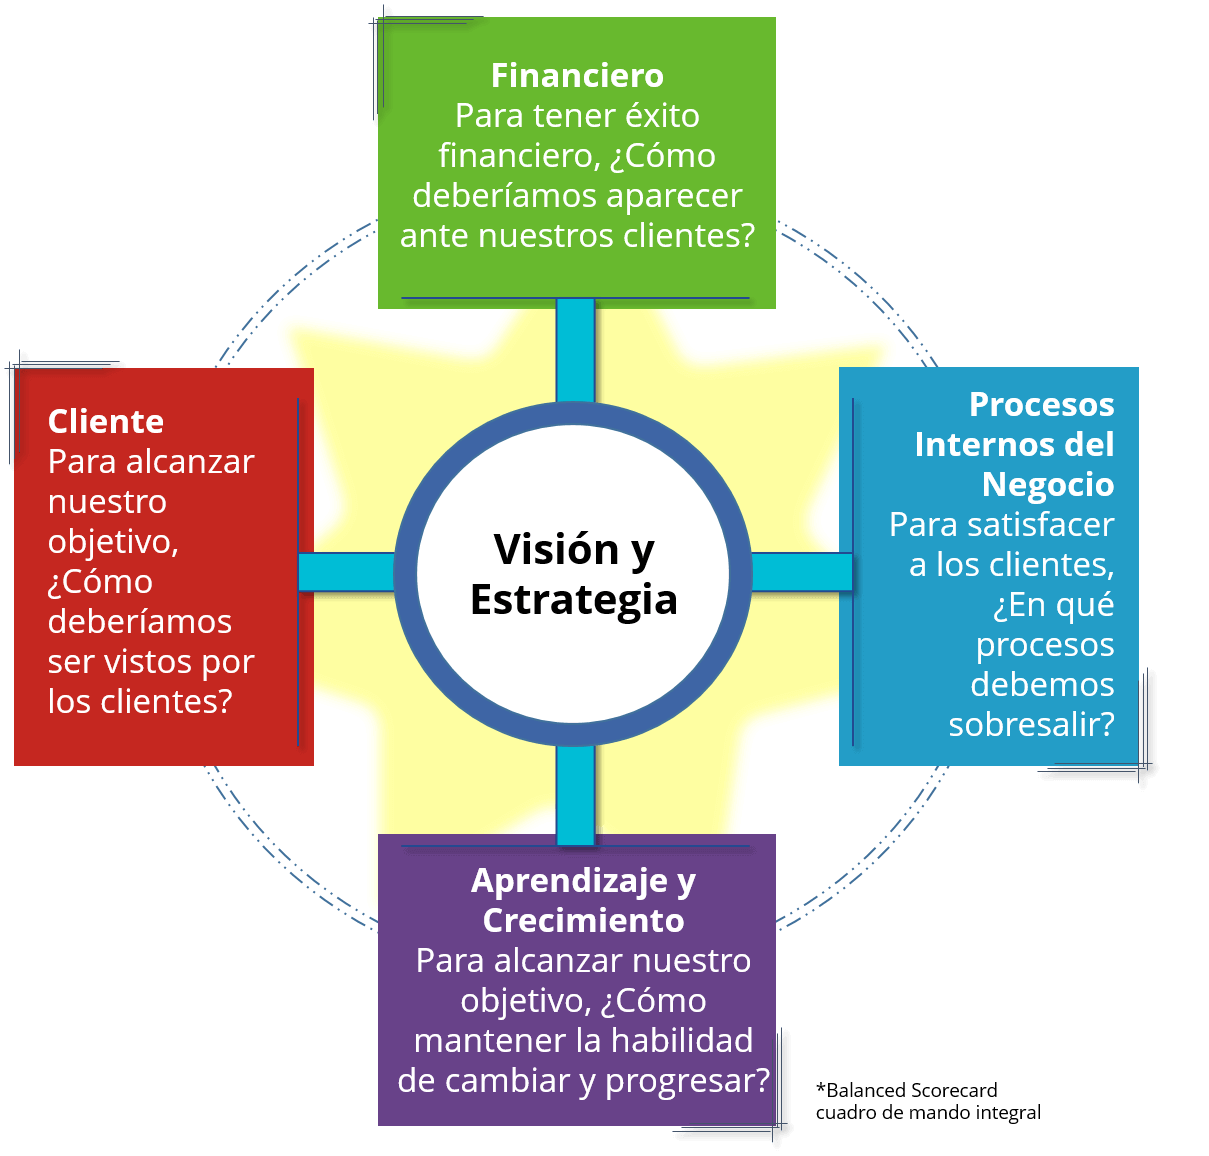
\includegraphics[width=15cm]{./Imagenes/imagen2}
\end{center}

\section{Beneficios}
\item{El Balanced Scorecard induce una serie de resultados que favorecen la administración de la compañía, pero para lograrlo es necesario implementar la metodología y la aplicación para monitorear, y analizar los indicadores obtenidos del análisis. Entre otros podemos considerar las siguientes ventajas:\\\\
-Alineación de los empleados hacia la visión de la empresa.\\
-Comunicación hacia todo el personal de los objetivos y su cumplimiento.\\
-Redefinición de la estrategia en base a resultados.\\
-Traducción de la visión y estrategias en acción.\\
-Favorece en el presente la creación de valor futuro.\\
-Integración de información de diversas áreas de negocio.\\
-Capacidad de análisis.\\
-Mejoría en los indicadores financieros.\\
-Desarrollo laboral de los promotores del proyecto.}

\begin{center}

\includegraphics[width=15cm]{./Imagenes/imagen3}
\end{center}

\section{Plan Estrategico}
\item{Es un proceso sistematico de desarrollo e implementacion de planes para alcanzar metas, propositos y objetivos.}

\item{ y debe:}
- Ser capaz de alcanzar el objetivo deseado
- Factible apropiada
- Debe proporcionar una ventaja compettitiva
- Capaz de adaptar a las situciones cambiantes
- Medible en terminos de su efectividad

\section{Modelo Canvas}
\item{
El modelo canvas es la herramienta para analizar y crear modelos de negocio de forma simplificada. Se visualiza de manera global en un lienzo dividido en los principales aspectos que involucran al negocio y gira entorno a la propuesta de valor que se ofrece.\\\\
El modelo canvas se utiliza para pasar de idea a proyecto y plasmar nuestra idea en un modelo empresarial. Es un modelo “vivo”, es decir, que vamos modificando según se va desarrollando, vamos validando clientes, surgen nuevas ideas… por eso se utilizan post-its para completarlo.
}

\section{Generar un modelo canvas}
\item{
Muestra de manera lógica la interconexión entre los 9 aspectos básicos de un modelo de negocio. A continuación, mostramos cómo se debe completar un modelo canvas, en qué orden y qué significa cada apartado del lienzo.\\\\
\textbf{1. Segmento de clientes}\\
Detectar las necesidades del mercado, del cliente. Nuestro foco siempre es el cliente y debemos orientar el producto a sus necesidades y deseos.\\
Para poder identificar a nuestro cliente debemos ponernos en su piel y analizar qué es lo que piensa, siente, ve, escucha, cuáles son sus problemas y los beneficios que le puede aportar nuestro producto/servicio.\\\\
Debemos dar respuesta a:\\
¿Para quién estamos creando valor?\\
¿Quiénes son nuestros clientes más importantes?
\\\\\textbf{2. Propuesta de valor}\\
Es la pieza clave de todo el modelo de negocio. La propuesta de valor o ventaja competitiva es el motivo por el que el cliente nos va a comprar a nosotros y no a otro. Aquí se incluye lo que hace diferente e innovador a nuestro producto/servicio.\\
Se puede innovar en diferentes aspectos como en el modelo de ingresos, alianzas empresariales, procesos productivos, entrega del producto/servicio, marca…\\\\
Debemos dar respuesta a:\\
¿Qué valor estamos entregando a nuestros clientes?\\
¿Qué problema resolvemos?\\
¿Cuál es la necesidad que satisfacemos?\\
¿Qué tipo de producto ofrecemos?\\\\
\textbf{3. Canales}\\
Una vez definidos nuestros clientes y la propuesta de valor que les ofrecemos, tenemos que llegar a ellos. Si no nos conocen, no nos van a comprar. Aquí vamos a definir los canales de distribución del producto o servicio.\\\\
Debemos dar respuesta a:\\
¿Con qué canales podemos llegar a nuestros clientes?\\
¿Qué canales funcionan mejor?\\
¿Cuáles de estos canales son los más rentables?\\\\
\textbf{4. Relación con los clientes}\\
Debemos comunicarnos correctamente con nuestros clientes y estar pendiente de ellos. Ellos son nuestro eje central, por lo que saber definir la relación que vamos a tener con cada segmento de clientes, es fundamental para el éxito de un negocio.\\\\
Debemos dar respuesta a:\\
¿Cuál es la relación que tenemos con cada uno de nuestros segmentos de clientes?\\
¿Qué tipo de relación esperan?\\
¿Qué coste tiene?\\\\
\textbf{5. Flujo de ingresos}\\
Para que un negocio sea rentable y podamos sobrevivir en el mercado, tenemos que pensar ¿Cómo monetizarlo? Es decir ¿De dónde vamos a obtener la facturación?\\\\
Debemos dar respuesta a:\\
¿Cuál es nuestra principal línea de ingresos? \\
¿Cómo pagarán nuestros clientes?\\
¿Por qué están dispuestos a pagar nuestros clientes?\\\\
\textbf{6. Recursos clave}
Conocer con qué recursos contamos y con los que debemos contar para llevar a cabo la actividad de nuestro negocio, es clave a la hora de establecer el plan de negocios. Debemos de ser cautos y prudentes a la hora de definir estos recursos. Siempre debemos pensar en la forma de optimizarlos, es decir, intentar conseguir la máxima productividad posible al mínimo coste.\\\\
Debemos dar respuesta a:\\
¿Qué recursos esenciales requiere nuestra propuesta de valor?\\\\
\textbf{7. Actividades clave}\\
Para llevar a cabo la propuesta de valor que queremos ofrecer a nuestros clientes, son necesarias ciertas actividades para preparar el producto antes de que llegue al mercado. Es decir, aquí pensamos en el core de nuestro negocio, lo que haremos en nuestro día a día.\\\\
Debemos dar respuesta a:\\
¿Qué actividad básica requiere nuestra propuesta de valor?\\
¿Cuáles son nuestros canales?\\
¿Cuáles son nuestras fuentes de ingresos?\\\\
\textbf{8. Aliados clave}\\
Para llevar a cabo un negocio, es imprescindible tener aliados. Estos aliados pueden ser;\\\\
Una serie de socios/colaboradores: una buena red de partners nos pueden ayudar a llegar más rápido al cliente, a ir avalados por su reputación y experiencia.\\
Los proveedores: aquellos que nos proporcionan los recursos clave para poder ofrecer los servicios/producto final.\\\\
Debemos dar respuesta a:\\
¿Quiénes son nuestros socios clave en el mercado?\\
¿Quiénes son nuestros proveedores?\\
\textbf{9. Estructura de costes}\\
Obviamente, toda esta infraestructura tiene unos costes que debemos pagar y optimizar. Debemos definir cuáles son nuestras prioridades y los gastos fundamentales en el negocio de aquellos que no lo son.\\
Tener bien clara esta estructura nos ayudará a no desviarnos de los presupuestos y que el negocio fracase por problemas de financiación.\\\\
Debemos dar respuesta a:\\\\
¿Cuáles son los costes más importantes dentro de nuestro modelo de negocio?\\
¿Qué recursos clave son los más costosos?\\
¿Qué actividades clave son las más costosas?\\
}
\begin{center}
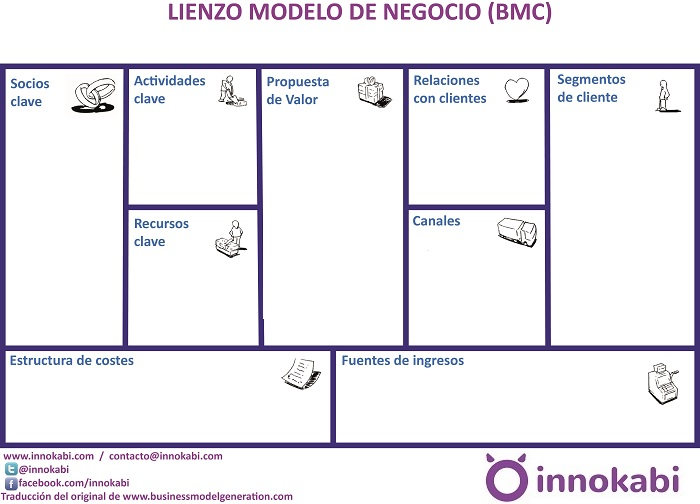
\includegraphics[width=15cm]{./Imagenes/imagen4}
\end{center}


\title{BALANCED SCORECARD EJEMPLO DE IMPLEMENTACIÓN EN UNA CORPORACIÓN EDITORIAL PARA MANTENER UNA POSICIÓN DE LIDERAZGO EN EL MERCADO}

\section{ANTECEDENTES Y JUSTIFICACIONES}
\item { Grupo Santillana Ecuador es una empresa de capitales españoles que ha liderado el sector editorial de texto escolar en Ecuador por los últimos 10 años. En este tiempo, se ha consolidado como la primera opción en el mercado escolar de textos de prescripción.

También ha logrado incursionar en nuevas unidades de negocios en los cuales tiene una participación representativa en el mercado nacional entre las que se destacan la comercialización de textos literarios para el público en general y servicios de capacitación a nivel de postgrado.}

\section{Su Estructura Comercial está conformada por cuatro líneas de negocio:}
\item { 1.-  Texto Escolar: es el sello con el cual edita y difunde textos y materiales para educación escolar.

2.- Richmond (Inglés): es el sello encargado de desarrollar y comercializar material didáctico para la enseñanza del idioma inglés para educación escolar.

3.- Ediciones Generales: comercializa libros de diversos sellos literarios que llegan al público lector para satisfacer la demanda de gran variedad de temas.

4.- Santillana Formación:  Es una nueva unidad de negocio que se divide en dos líneas de servicios:

1. Instituto Universitario de Postgrados – IUP: Convenio con universidades españolas que le acredita a Santillana desarrollar programas de postgrados que permitan a profesionales ecuatorianos acceder a maestrías internacionales.

2. Santillana Profesional: diseño de proyectos educativos mediante modernas tecnologías (e – learnig).}

\begin{center}
\includegraphics[width=15cm]{./Imagenes/ImgEmpresa1.png}
\end{center}

\item { A pesar del éxito obtenido en los últimos años, Santillana ha visto la necesidad de buscar nuevas estrategias y mecanismos de gestión  para mantener esa posición de liderazgo frente a la creciente y agresiva competencia en todas sus líneas de negocio.

Especialmente en la que consideran su bastión, texto escolar, que constantemente se ve amenazado por empresas rivales que copian y anulan muchas de las estrategias comerciales implementadas.}

\section{BALANCED SCORECARD EJEMPLO DE HERRAMIENTA: POR QUÉ RAZÓN ELIGIERON USAR UN TABLERO DE COMANDO}
\item { Con este antecedente y luego que a finales del 2004 se definiera el Plan Estratégico de la organización que contempla objetivos claves que deben cumplirse hasta el año 2009, se decidió implementar una herramienta de control estratégico como el BSC para darle seguimiento a la estrategia, y proyectos para cumplir los propósitos establecidos.

En este proceso, surgió la pregunta ¿Cómo hacer para que los planes de la Organización dejen de ser planes y se conviertan en realidad?

El primer paso para responder a esta pregunta es tener en cuenta que los activos intangibles conforman el mayor valor de toda Organización y que ninguna estrategia daría resultados positivos si no se le da el seguimiento apropiado.

Se decidió utilizar el Balance Scorecard debido a los beneficios que proporciona involucrando a los activos intangibles con su relación de desempeño. Además que el rápido retorno de la inversión estimada inclinaban ciertamente la utilización de esta herramienta.

Se estimó que luego de la implementación, cuando esté en explotación todo el sistema, los logros que se obtengan motivarán a seguir realizando nuevas mejoras en la organización. Con ello, a más darle seguimiento a la estrategia y de lograr un retorno de la inversión en un corto plazo, se logran fortalecer algunas debilidades que se identificaron en la empresa. Entre las más destacables:

1. Mejorar el sistema de comunicación interno
2. Disciplinar al personal
3. Crear cultura de medición y consecución de objetivos.
4. Establecer mecanismos de retroalimentación para mejoras

Otro factor que influyó en tomar la decisión de utilizar el Scorecard como herramienta de gestión estuvo relacionado con la administración y seguimiento de las diversas áreas de negocios con las que cuenta actualmente la empresa.

En vista de que se cuenta con cuatro unidades de negocios, 3 de ellas bien diferenciadas, se estableció como necesidad delinear estrategias distintas y segmentadas para cada una de ellas, las mismas que se deberían estar alineadas con la estrategia corporativa global de crecimiento financiero fijada por la matriz.}

\section{BALANCED SCORECARD EJEMPLO DE IMPLEMENTACIÓN}
\item {El proceso de implementación en Grupo Santillana inició luego de validar  el plan estratégico acordado hasta el 2009, y se estableciera un ROADMAP a seguir para cubrir la brecha entre la situación actual y la deseada en ese umbral de tiempo.

En este mapa de camino, se establecen claramente los pasos a seguir y nos da un estimado de tiempo para su consecución (un mes por cada uno de las fases):}

\begin{center}
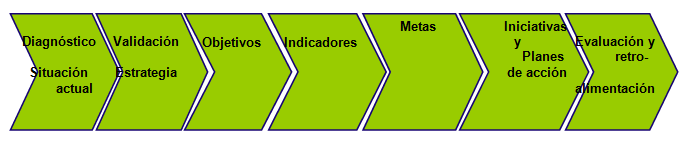
\includegraphics[width=15cm]{./Imagenes/ImagenEmpresa2.png}
\end{center}



\newpage
\begin{center}
\vspace*{0.1in}
\begin{Large}
\section{BALANCED SCORECARD EJEMPLO DE IMPLEMENTACIÓN} \\
\end{Large}
\end{center}


\item {El proceso de implementación en Grupo Santillana inició luego de validar  el plan estratégico acordado hasta el 2009, y se estableciera un ROADMAP a seguir para cubrir la brecha entre la situación actual y la deseada en ese umbral de tiempo.

En este mapa de camino, se establecen claramente los pasos a seguir y nos da un estimado de tiempo para su consecución (un mes por cada uno de las fases):}
\subsection{Balanced Scorecard Ejemplo de Implementación – Paso 1}
\item {Definir el Mapa Estratégico Corporativo y Validación de la Estrategia

Clarificar la Visión definida por la empresa en el Plan Estratégico fue la primera de las actividades realizadas, debido a que de ahí se derivan el resto de componentes del scorecard.

Formular la hipótesis estratégica (seleccionar los temas estratégicos) se hizo conjuntamente con la validación de la visión de la empresa y surgieron algunas dudas que se fueron aclarando y puliendo hasta obtener el cuadro de mando corporativo, que sería la base de nuestro scorecard.

Esta estrategia global fue “bajada” a un segundo nivel para trabajarla por cada unidad de negocio, por lo que cada unidad trabajó en su propuesta de valor única para su segmento específico de clientes, con los cuales se desarrollo esa combinación de producto, calidad de servicio, precio, e imagen que se ofrece a los clientes para distinguirse de la competencia.

El cuadro de mando para Santillana se lo trabajó en 2 niveles de los 3 posibles, al nivel gerencial o mandos altos, y al nivel de mandos medios, se dejó de lado por esta ocasión el cascadearlo hasta el nivel operativo por motivo de recursos y tiempo. Sin embargo, existe la intención de abarcar este nivel en un futuro cercano una vez que el esquema de remuneración variable también sea habilitado.

El mapa aquí presentado es claro y nos demuestra las relaciones causa y efecto entre cada perspectiva, tratando de armonizar con el cuadro de mando que se maneja bajo la misma filosofía, dado que no es posible buscar las respuestas al desempeño financiero en la misma perspectiva sino en su concatenación con el resto de áreas que directamente influyen en esos resultados. El objetivo fue no perder el concepto de integralidad.}

\begin{center}
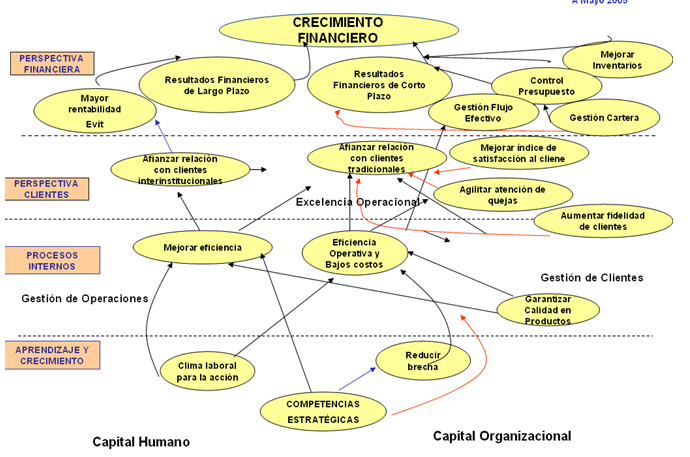
\includegraphics[width=15cm]{./Imagenes/ImagenEmpresa3.png}
\end{center}

\subsection{Balanced Scorecard Ejemplo de Implementación – Paso 2: Objetivos Estratégicos Corporativos por Perspectiva}
\item {1. Se trabajó en establecer “Propuesta de Valor” por cada segmento de clientes. Entre los cuales deberíamos diferenciar por unidad de negocio, por estrato social y por capacidad de consumo. En todos ellos se acordó que la propuesta ganadora estaría principalmente enfocada en tener una mayor intimidad con el cliente, para conocerlo mejor y de esa forma poder adaptar nuestra oferta a sus gustos.

2. Definir los objetivos de contribución para cada perspectiva y objetivos estratégicos establecidos.  Este fue un factor importantísimo dado que con cada gerente de área se trabajo detenidamente para determinar en qué forma su área podía alinearse con los objetivos estratégicos corporativos ya definidos. Se lograron importantes análisis que se incluyeron como aportes de cada área, los cuales fueron luego llevados a iniciativas y planes de acción.

3. Identificación de los procesos de gestión críticos para alcanzar la estrategia
Se identificaron cuales procesos se consideraban críticos para alcanzar lo propuesto, luego de varias charlas y análisis conjunto entre los gerentes de área, se acordó que implementar un sistema de control y atención de quejas y otro de información para fidelidad y retención.

Para ayudarnos a identificar estos procesos se recurrió muchas veces a sencillas preguntas como:

* Qué necesidades de información no han sido satisfechas
* Por qué hacemos las cosas de esta forma y no de otra
* Qué vacíos encontramos en los procesos actuales
* Por qué no hemos enfrentado este problema con anterioridad
* Cómo podemos mejorar esa área
* Qué necesitamos para fortalecer nuestras debilidades
* Qué se nos pasó por encima.}






\subsection{alanced Scorecard Ejemplo de Implementación – Paso 3: Identificación de Competencias, habilidades y formación del personal}
\item {En este proceso también se determinó que para alcanzar los objetivos propuestos era indispensable contar con personal bien capacitado y formado. Se determinó que no solamente era necesario involucrar a los directores sino también, y en muchos casos obligadamente, al personal operativo que tiene relación directa con los clientes. Por lo que se establecieron programas de formación para el personal en varias doctrinas y para estos empleados, charlas de servicio al cliente.}

\subsection{Balanced Scorecard Ejemplo de Implementación – Paso 4: Identificación del Capital de la Información.}
\item {Considerando que la información es vital para la toma de decisiones, se decidió impulsar proyectos de Análisis Multidimensional de la información para la toma de decisiones. Gracias a la implementación paralela de herramientas de software de Business Intelligence (Olaps) y reporteadores Gerenciales, se logro automatizar de gran forma el acceso a información considerada crítica.

El uso de estas herramientas estuvo acompañado de igual forma de charlas de capacitación sobre los productos en sí y sus beneficios.}

\subsection{Balanced Scorecard Ejemplo de Implementación – Paso 5: Indicadores estratégicos Corporativos}
\item {* Identificar inductores de actuación del personal para alcanzar los objetivos. Con la implementación de cada indicador se relacionaban los inductores de actuación esperados para el desempeño del personal.

* Análisis de Indicadores: qué, quien, cómo, cuándo. El análisis y validación de indicadores bajo las perspectivas de: contribución, factibilidad de obtención, y precisión.

* Validar correlación y relación causa efecto de indicadores fue la tercera tarea propuesta en este proceso. Quizás resulto ser uno de los más extensos debido a que se debió analizar uno a uno su relación con otros indicadores y sus otras posibles correlaciones. En este proceso se ha tratado de integrar las diferentes perspectivas propuestas por Norton y Kaplan en la medida que ha sido posible, sin embargo quizás no este del todo de esa forma, pero principalmente se ha querido potencializar el valor de los activos intangibles: capital humano, capital organizacional y capital de información. Para lograr que estos intangibles se convierten en resultados tangibles.}

\subsection{Balanced Scorecard Ejemplo de Implementación – Paso 6: Metas Corporativas}
\item {* Análisis de las metas establecidas. Se realizó un análisis global de las metas establecidas en el plan estratégico y como ellas deberían ser conseguidas año tras año, período de medición tras período.  Este proceso tomó de igual forma bastante tiempo debido a que el proceso de fijación de metas resulta un poco complejo dependiendo del tipo de empresas con las que se trabaje.

* Definición de  metas de mediano y largo plazo

* Para cada área se definieron las metas a mediano plazo que deberían estar coherentes con las metas corporativas ya establecidas.}

\subsection{Balanced Scorecard Ejemplo de Implementación – Paso 7: Iniciativas estratégicas}
\item {* Validar iniciativas actuales  (Análisis vertical por Objetivo) y por actores (Análisis Horizontal)

* Se realizó la validación de cientos de iniciativas por las dos vías conocidas por aporte a los objetivos estratégicos y por actores involucrados. En este proceso y luego de la validación se depuraron muchas iniciativas que verticalmente no tenían muchas coincidencias de alineación, dándoles por supuesto prioridad a quellas que cumplían con al menos 2 coincidencias.

* Matriz para la priorización de iniciativas.

* De igual forma como se realizo con los indicadores, la priorización de iniciativas estuvo basada en 3 aspectos fundamentales: contribución al objetivo, factiblidad y relación costo beneficio.}

\subsection{Balanced Scorecard Ejemplo de Implementación – Paso 8: Desarrollo de umbrales}
\item {* Definir los límites de control para cada una de las metas establecidas fue más sencillo ya que se estandarizó en la herramienta valores fijos en porcentajes. Este proceso ahorro tiempo debido a que al estandarizar los umbrales cada uno de los involucrados en el proceso conocía que su rendimiento iba a ser monitoreado bajo el siguiente parámetro de semáforos.}
\begin{center}
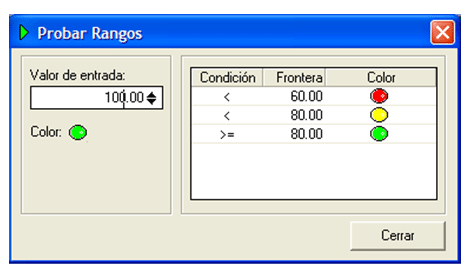
\includegraphics[width=15cm]{./Imagenes/img01.png}
\end{center}
\subsection{Balanced Scorecard Ejemplo de Implementación – Paso 9: Desarrollo y despliegue el Cuadro de Mando Integral}
\item {* Este fue ya el proceso final de toda la implementación, en el cual luego de validarlo y aprobarlo por todas las áreas de la empresa en consenso se lo decidió subir a una herramienta de software especializada en el manejo de indicadores para que se facilite su ejecución y monitoreo.

* En la figura adjunta se aprecia parte (debido a que es extenso el modelo) de cómo luce el tablero de comando en la empresa. Lo interesante de destacar en este modelo es que se han incluido todas las sugerencias y aspiraciones del personal de la empresa y se han alineado todas las áreas de la organización. Por lo que cada uno puede fácilmente responder por los resultados de su gestión, personal o del área.}
\begin{center}
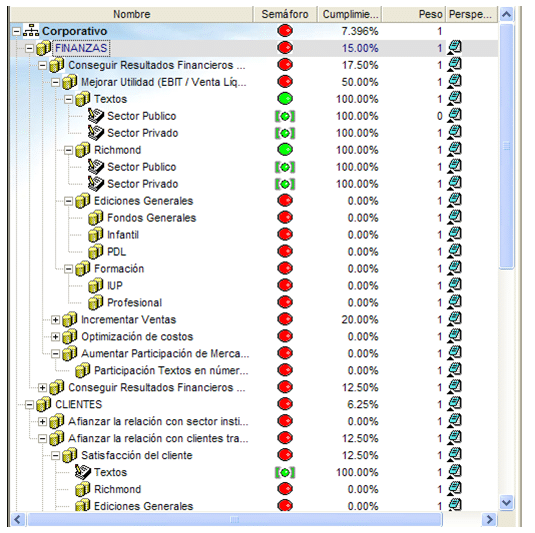
\includegraphics[width=15cm]{./Imagenes/img02.png}
\end{center}



\begin{center}
\vspace*{0.1in}
\begin{Large}
\section{BALANCED SCORECARD EJEMPLO DE HERRAMIENTA: QUÉ DIFICULTADES TUVIERON EN EL DISEÑO E IMPLEMENTACIÓN DEL TABLERO DE COMANDO} \\
\end{Large}
\end{center}

\item {El proceso de diseño e implementación, como todo nuevo proyecto, presentó algunas dificultades, relacionadas principalmente con involucrar a una gran cantidad de actores. En vista del gran número de áreas, unidades de negocios, responsables y objetivos, tomo algún tiempo el alcanzar consensos para delinear sus componentes. Entre las principales dificultades encontradas podemos destacar:}

\subsection{Comunicación}
\item {El proceso comunicativo de Grupo Santillana hasta la implementación del BSC estaba muy centralizado en directores y gerentes de área, por lo que el resto del personal, poco o nada conocía sobre los direccionamientos que tomaba la corporación. El comenzar a inculcar reuniones periódicas y boletines informativos para el resto del personal de la empresa, ha sido un proceso que ha tomado tiempo pero que está dando resultados importantísimos.}

\subsection{Trabajo en Equipo}
\item {Uno de los más comunes problemas que se encuentran durante estos procesos de implementación es el que “cada uno defiende lo suyo”, por lo que se trató de evitar la política de que cada uno defiende su trabajo independientemente de lo que suceda con la organización, lo que por lo general se traduce en reacciones poco positivas como atacar a otras áreas sin obtener la visión de que este proceso es una responsabilidad de todo el equipo gerencial y no de las áreas funcionales.

El proceso de alineación en el cual se ve envuelto Grupo Santillana, luego de la definición de su scorecard,  ha abarcado el trabajo en equipo de diferentes áreas, el poder admirar a la organización desde un punto de vista más holístico genera que se enfrenten muchas falencias que se pasaban por desapercibido. De igual forma el sensibilizar que este proceso es un trabajo de todos y para todos, no solo de los mandos superiores ha contribuido a cambiar esas viejas costumbres grupistas.}

\subsection{Liderazgo}
\item {El líder tiene un papel protagónico en el proceso de implantación de las estrategias en la empresa, por el pensamiento estratégico y la actitud estratégica que son indispensables para encaminar estos proyectos.

Es un factor crítico que tomó algún tiempo para poder desarrollarlo, para que cada jefe de área sea finalmente quienes sigan impulsando el modelo a sus subalternos, pero el haberlo hecho consolida la continuidad del proyecto. Si bien desde el inicio hubo la voluntad de todos y la decisión de gerencia general para emprender con este nuevo sistema de gestión, la verdadera aplicación de los mismos tomó tiempo, horas de sensibilización y capacitación, para que obtengan los resultados esperados.}

\subsection{Falta de enfoque}
\item {En muchas de las nuevas líneas de Grupo Santillana, la poca claridad de un enfoque sobre su mercado meta y el tipo de relación que deberían tener ocasionó más de una dificultad. Principalmente se hace difícil en Corporaciones con distintas líneas de productos el poder unificar una estrategia comercial común bajo un mismo enfoque, luego de las reuniones con los representantes de estás áreas.

Ha sido un largo proceso hasta que la Organización definió con claridad la estrategia que seguirá en el mediano plazo (entre tres y cinco años).

Durante las charlas y talleres se logró explicar la esencia de La estrategia,  es decir lo que debe hacer la Organización para llegar de un punto de referencia inicial, que es la situación actual, al punto de referencia final o situación deseada.

Se inculcó mucho a esencia de la planeación estratégica, para la selección de actividades que la Organización realizará para cerrar la brecha entre situación actual y situación deseada, en escoger realizar actividades diferentes a las realizadas por la competencia, o realizar las mismas actividades de una manera distinta.

Se llegó a determinar que quizás el mayor problema no era definir la estrategia sino como implementarla, como involucrar a todo el personal en ese proceso con responsabilidad y compromiso. Ese era un reto al que se debería llegar.

Tratar de alcanzar una estrategia ganadora que realmente marque una diferencia frente a la competencia.

El objetivo de esta implementación será que luego de algunos años no solamente queden los indicadores y metas como referencia de lo que se hizo, sino más bien que no se pierda la hipótesis planteada en la estrategia y sus relaciones de causa y efecto.

Se ha querido hacer énfasis en la relación causa efecto entre perspectivas para que realmente de una connotación de un verdadero scorecard.}

\subsection{Opiniones divergentes y diversas}
\item {Como en toda organización liderada por seres humanos, la gran cantidad de opiniones y puntos de vista de los responsables del área, hizo que se desarrollen y se desmenucen muchos de los requerimientos e inquietudes previo a la definición de indicadores.

Si bien la base del proceso fue la alineación de cada área con los respectivos objetivos estratégicos definidos con anterioridad se trabajó mucho para ir ajustando cada área a lo que la estrategia requería.

En este proceso también se incluyeron muchas sugerencias de parte de cada área para satisfacer la forma en cómo querían ser medidos y evaluados.}


\subsection{Débil definición de procesos y o procedimientos (en algunas áreas)}
\item {En este proceso de implementación del BSC, se encontró que existen escasos procedimientos y procesos definidos para algunas áreas, por lo que fue motivo de analizarlos y fortalecerlos con el fin de que sean parte de la estrategia corporativa.

Esto tomó tiempo y aplazó algunos hitos definidos en los cronogramas, pero finalmente la aclaración de cómo manejar algunas áreas (especialmente reclamos) fue un factor importantísimo para la organización.}

\subsection{Débil definición de procesos y o procedimientos (en algunas áreas)}
\item {Si bien actualmente Grupo Santillana cuenta con un sistema transaccional de información, no cubre en gran porcentaje la demanda de información de las diversas áreas.

Más aún cuando se tienen 2 aplicaciones adicionales que complementan la información de mercado y muchas veces esa información crítica de perfiles de clientes solamente se encuentra registrada manualmente en informes de los delegados comerciales.

En este aspecto, se desarrollaron algunos cubos dinámicos de información, y reportes inexistentes hasta la fecha para llenar estos vacíos. Adicionalmente se establecieron procedimientos para que cada uno de los responsables de cada área solicite reportes y cubos de análisis a sistemas para la toma de decisiones.}


\subsection{Poca cultura en el uso de indicadores y definición de metas}
\item {Un factor que ha sido una barrera importante para trabajar y avanzar en el proceso ha sido la poca cultura del empleado de trabajar en base a objetivos, consecución de metas y evaluación.

Esto se ha ido limando con constantes charlas de capacitación que han logrado persuadir de los beneficios de establecer mecanismos de control y medición como los que ofrece el Scorecard.}

\subsection{Fuerte orientación hacia cumplimiento de presupuestos financieros}
\item {Grupo Santillana es una corporación que ha tenido un vínculo muy fuerte hacia el seguimiento y cumplimiento de los presupuestos formulados por su casa matriz. En la nueva administración propuesta luego de la implementación, si bien el manejo presupuestario es considerado, no es el único mecanismo de evaluación.

Ese paradigma y costumbre poco a poco se está viendo cambiada por la nueva propuesta de gestión bajo indicadores no financieros.

Durante el proceso de alineación nos encontramos con algunas dificultades, el pensar en forma estratégica y sistémica hace que inducir a varios componentes de la organización en torno a la estrategia sea un proceso que se lo hace detenidamente para evitar confrontaciones.}

\subsection{Rotación de personal en algunas áreas claves}
\item {El hecho de que este proceso sea considerado a corto plazo y se trabaje bajo presión ha incidido en la rotación de personal. De igual forma el cambio de estructuras internas definidas por matriz son algunos factores críticos que han dificultado el avance del proceso.

Debido a que, al cambiar la estructura y la función de uno u otro departamento, cambia indiscutiblemente la forma en cómo será evaluado y bajo que perspectiva se alineará en el cuadro de mando. De igual forma la rotación de personal en algunas gerencias y/o el cambio de funciones de algunos empleados claves, dio un giro a lo que ya se estaba definiendo.

Como es de esperarse los cambios exigidos por la matriz también influyen en la forma de cómo se despliega el scorecard dentro la organización. Esto ha influido en que ha tomado un poco más de tiempo hasta aclarar estos puntos.}




\begin{center}
\vspace*{0.1in}
\begin{Large}
\section{BALANCED SCORECARD EJEMPLO DE HERRAMIENTA: QUÉ BENEFICIOS LOGRARON A PARTIR DE LA IMPLEMENTACIÓN} \\
\end{Large}
\end{center}

\item {Gracias al apoyo del capital intelectual del valioso personal de la organización y el uso de herramientas tecnológicas de soporte para la toma de decisiones, se agilitarán algunos procesos, se reestucturarán otros, se reducirán costos, se ofrecerá una propuesta de valor significativa al cliente y finalmente las decisiones serán más asertivas en base a datos reales.

El aplicar la metodología y alcanzar los objetivos estratégicos de corto y largo plazo sin duda mantendrán el liderazgo en el texto escolar, crecimiento en el sector formativo y diversificación en el de fondos generales.

Es por ello que conjuntamente con la implementación de esta herramienta se han emprendidos proyectos para fortalecer las Competencias de los principales  ejecutivos y colaboradores, cuyo objetivo final será ligar la evaluación del desempeño a los resultados obtenidos, para que de alguna forma se de continuidad a este proceso.

Durante el proceso de implementación se han logrado identificar unos cinco beneficios que creemos son claves en este proceso.

* Nadie es dueño de la verdad

Un factor que consideramos que ha sido importantísimo es el saber escuchar las opiniones de terceros, nos dimos cuenta que en este tipo de procesos todos somos facilitadotes y que por más experiencia que tengamos en uno u otro campo, no somos dueños de la verdad, esta puede tener muchas aristas que deben ser consideradas para el bien de la organización. Nos ha enseñado a aprender a escuchar, aceptar y tolerar las opiniones de terceros.

* Es un proceso de mejora continua

Otro gran beneficio que se encontró en este proyecto es que si bien se definió ya un modelo estratégico y de tablero de comando, eso no quiere decir que sea inmodificable.  Todos estuvimos de acuerdo que para esta primera etapa y para familiarizarnos era el más adecuado, pero que muy probablemente se lo pudiera ir mejorando, cambiando con el tiempo. Nos dimos cuenta que es un proceso continuo y nunca termina de implementarse, y que cada vez lo podemos hacer más retador.

* Involucra a todo el personal

Otro beneficio sustancioso ha sido que este proceso ha involucrado directamente a todo el personal de la empresa, al menos desde los mandos altos hasta los mandos medios. Quienes tienen el compromiso de seguir trabajándolo hasta llegar a los niveles operativos. Ha sido una gran oportunidad para que muchos opinen y sean parte de este cambio.

* Desarrollo de  actitudes (proactividad) y cultura de medición y evaluación.

Un factor útil que se ha obtenido con la implementación de esta herramienta es concientizar al personal de los beneficios de trabajar bajo esta metodología, lo cual facilita adoptar nuevos compromisos frente a las obligaciones.

Que conozcan que van a ser medidos y evaluados bajo este proceso es un desafío que a pesar que ha tomado tiempo y se tiene que ir insistiendo en el tema ya se ha forjado un camino que se debe seguir.

El desarrollo de esa actitud proactiva ha sido beneficioso para prepararnos frente a los cambios externos que pudieran afectar nuestra organización, lo que nos ha fortalecido internamente, brindándonos más seguridad y confianza en lo que hacemos.

Nos permite visualizar en 5 minutos la situación de la empresa.

Las reuniones ahora son mucho más ejecutivas y cortas, solamente basta que cada uno revise tu tablero de comando y en apenas 30 minutos se discuten los objetivos no cumplidos, las metas no alcanzadas o las iniciativas pendientes. Las reuniones se enfocan en los aspectos que necesitan ser mejorados o corregidos. Todos sienten ser parte de esa estrategia.
}


\begin{center}
\vspace*{0.1in}
\begin{Large}
\section{BALANCED SCORECARD EJEMPLO DE HERRAMIENTA: QUÉ RECURSOS INVIRTIERON (GENTE, DINERO, TIEMPO)} \\
\end{Large}
\end{center}

\item {Entre los principales recursos invertidos en este proyecto se deben destacar en el siguiente orden:}


\subsection{Personal}
\item {Se ha invertido mucho en el personal, no solo en la capacitación de la metodología, la herramienta y sus beneficios, sino en su formación para complementar su perfil de competencias. Este hecho no solo es beneficiosos para este proyecto sino para el resto de actividades que tienen que emprender bajo sus funciones.}

\subsection{Tiempo}
\item {El recurso tiempo ha sido vital debido a que se ha dedicado gran cantidad de tiempo por parte de todos los actores en el proceso hasta lograr el objetivo final. Este proceso no ha resultado complicado pero sí demoroso dado el nivel de control al cual se ha querido llegar y el nivel de involucramiento necesario del personal para ir definiendo poco a poco el modelo.}

\subsection{Dinero}
\item {En el aspecto económico, si bien se ha invertido dinero para automatizar algunos procesos, para la implementación de herramientas de análisis multidimensional y el monitoreo de la estrategia, ha resultado un valor marginal frente a los otros beneficios que se están obteniendo. Por lo que se espera el retorno de la inversión de este proyecto en un corto plazo, aproximadamente un año.}

\newpage
% Bibliografía.
%-----------------------------------------------------------------
\begin{thebibliography}{99}
https://www.isotools.org/2015/02/23/que-es-el-balanced-scorecard-conoce-su-funcionamiento-y-ventajas/\\
https://economipedia.com/definiciones/modelo-canvas.html\\
http://www.infoviews.com.mx/Bitam/ScoreCard/]\\
https://innokabi.com/canvas-de-modelo-de-negocio/\\
https://josefacchin.com/modelo-canvas-de-negocio/\\
https://www.adaptiveus.com/balanced-scorecard-vs-business-model-canvas/\\

\bibitem{Cd94} Autor, \emph{Título}, Revista/Editor, (año)

\end{thebibliography}

\end{document}
